\documentclass[12pt]{standalone}
\usepackage{amsmath, relsize, tikz}
\usepackage{xcolor}
\usepackage{pgffor} % LATEX
\input pgffor.tex % plain TEX
\usetikzlibrary{matrix}
\usetikzlibrary{knots}
\usetikzlibrary{intersections,backgrounds}
\usetikzlibrary{patterns}
\begin{document}
    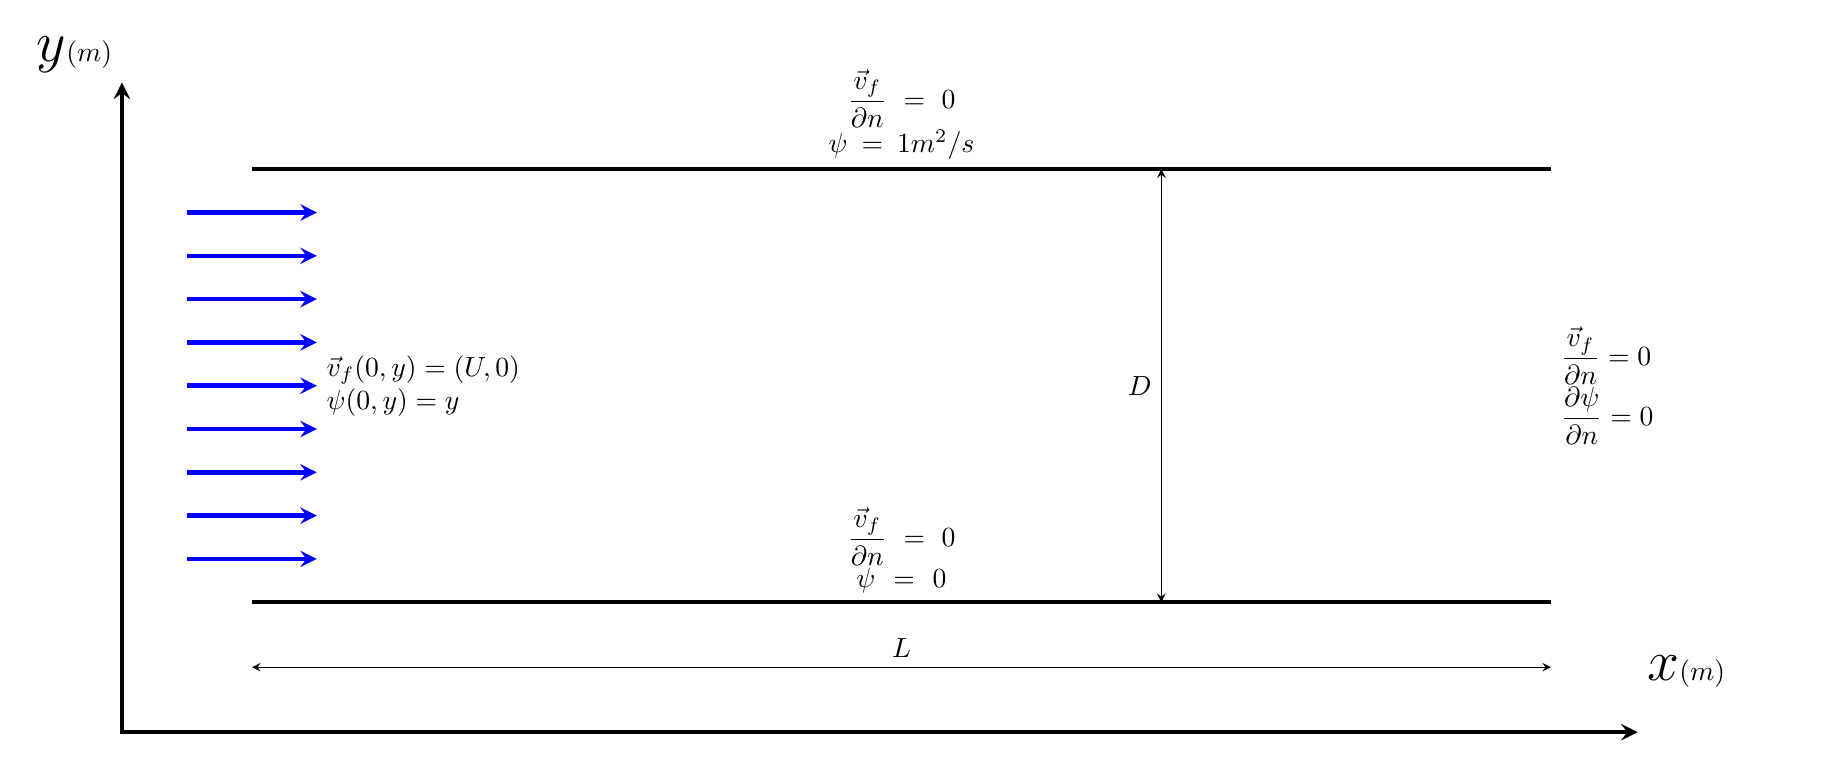
\begin{tikzpicture}[scale=5.5, >=stealth]
        \draw [ultra thick] (0, 1) -- (3, 1);
        \draw [ultra thick] (0, 0) -- (3, 0);
        \draw [<->, ultra thick] (-0.3,1.2) -- (-0.3,-0.3) -- (3.2,-0.3);

        \node [above left] at (-0.3,1.2) {{\huge $y$}{$(m)$}};
        \node [below right] at (3.2,-0.1) {{\huge $x$}{$(m)$}};

        \node [above, text width=3cm, align=center] at (1.5, 1) {$\dfrac{\vec{v}_f}{\partial n} = 0$\\$\psi = 1m^2/s$};
        \node [above, text width=3cm, align=center] at (1.5, 0) {$\dfrac{\vec{v}_f}{\partial n} = 0$\\$\psi = 0$};
        \node [right, text width=3cm] at (0.15, 0.5) {$\vec{v}_f(0,y) = (U,0)$\\$\psi(0,y) = y$};
        \node [right, text width=3cm] at (3, 0.5) {$\dfrac{\vec{v}_f}{\partial n} = 0$\\$\dfrac{\partial \psi}{\partial n} = 0$};

        \draw [<->] (0.0, -0.15) -- (3.0, -0.15);
        \node [above] at (1.5, -0.15) {$L$};
        \draw [<->] (2.1, 0.0) -- (2.1, 1.0);
        \node [left] at (2.1, 0.5) {$D$};

        \foreach \y in {0.1, 0.2, ..., 0.9}
        {
            \draw [blue, ->, ultra thick] (-0.15, \y) -- (0.15, \y);
        }
    \end{tikzpicture}
\end{document}


